\chapter{Fundamentals of USB Power Delivery}

The field of power delivery and charging technologies has witnessed significant advancements in recent years, driven by the proliferation of portable electronic devices and the demand for faster, more efficient charging solutions. Among these developments, \gls{usbpd} stands out as a critical standard that has reshaped the landscape of device connectivity and power management.

In this chapter, we delve into the foundational principles underlying USB PD, exploring its origins, key components, and operational mechanisms.

\section{Overview of USB Power Delivery}
 \begin{table}[htb]
    \centering
    \caption{USB Specifications and Their Maximum Voltage, Current, and Power}
    \label{tab:usb_specifications}  
    \begin{tabular}{|l|c|c|c|}
        \hline
        \textbf{Specification} & \textbf{Maximum voltage} & \textbf{Maximum current} & \textbf{Maximum power} \\
        \hline
        USB 2.0 & 5 V & 500 mA & 2.5 W \\
        \hline
        USB 3.0 and USB 3.1 & 5 V & 900 mA & 4.5 W \\
        \hline
        USB BC 1.2 & 5 V & 1.5 A & 7.5 W \\
        \hline
        USB Type-C 1.2 & 5 V & 3 A & 15 W \\
        \hline
        USB PD 3.0 & 20 V & 5 A & 100 W \\
        \hline
    \end{tabular}
    
\end{table}
The Universal Serial Bus (USB) has undergone a significant evolution since its inception. Initially, it was designed as a data interface with the capability of supplying limited power. This was sufficient for early peripherals like keyboards and mice, but as the USB ecosystem expanded to include devices like printers, scanners, and external hard drives, the power supply aspect became increasingly important. 

With the advent of USB Power Delivery (PD), USB transformed from being just a data interface to a primary provider of power. This was a major shift in the USB paradigm, enabling it to power and charge power-hungry devices such as laptops, monitors, and docking stations \cite{Truechip2024}. The USB PD specification introduced more flexibility with a new reversible USB-C connector, more protocols, and increased speed with USB 3.1.

Table\ref{tab:usb_specifications} provides a comparative analysis of different USB specifications in terms of their maximum voltage, current, and power capabilities. This comparison is crucial for understanding the evolution and advancements in USB technology, particularly in the context of power delivery.

Starting with USB 2.0, it has a maximum voltage of 5V, a maximum current of 500mA, and a maximum power output of 2.5W. This specification was sufficient for early USB devices like keyboards and mice, which required minimal power.
USB 3.0 and 3.1 specifications also maintain a maximum voltage of 5V but increase the maximum current to 900mA, resulting in a maximum power output of 4.5W. This enhancement allowed for faster data transfer rates and supported more power-hungry devices compared to USB 2.0.

The USB Battery Charging (BC) 1.2 specification further increases the maximum current to 1.5A while keeping the voltage at 5V, leading to a maximum power output of 7.5W. This specification was designed to improve charging times for devices like smartphones and tablets.

USB Type-C 1.2 introduces a significant improvement with a maximum current of 3A at 5V, resulting in a maximum power output of 15W. The USB Type-C connector is reversible and supports higher power delivery, making it more versatile for modern devices.

Finally, USB Power Delivery (PD) 3.0 represents the most advanced specification in the image. It supports a maximum voltage of 20V and a maximum current of 5A, allowing a maximum power output of 100W. This specification enables USB to power larger devices such as laptops and monitors, showcasing the evolution of USB from a simple data interface to a robust power delivery system.

\section{Principles of Operation}
\subsection{USB Type-C}
\begin{figure}[htb]
    \centering
    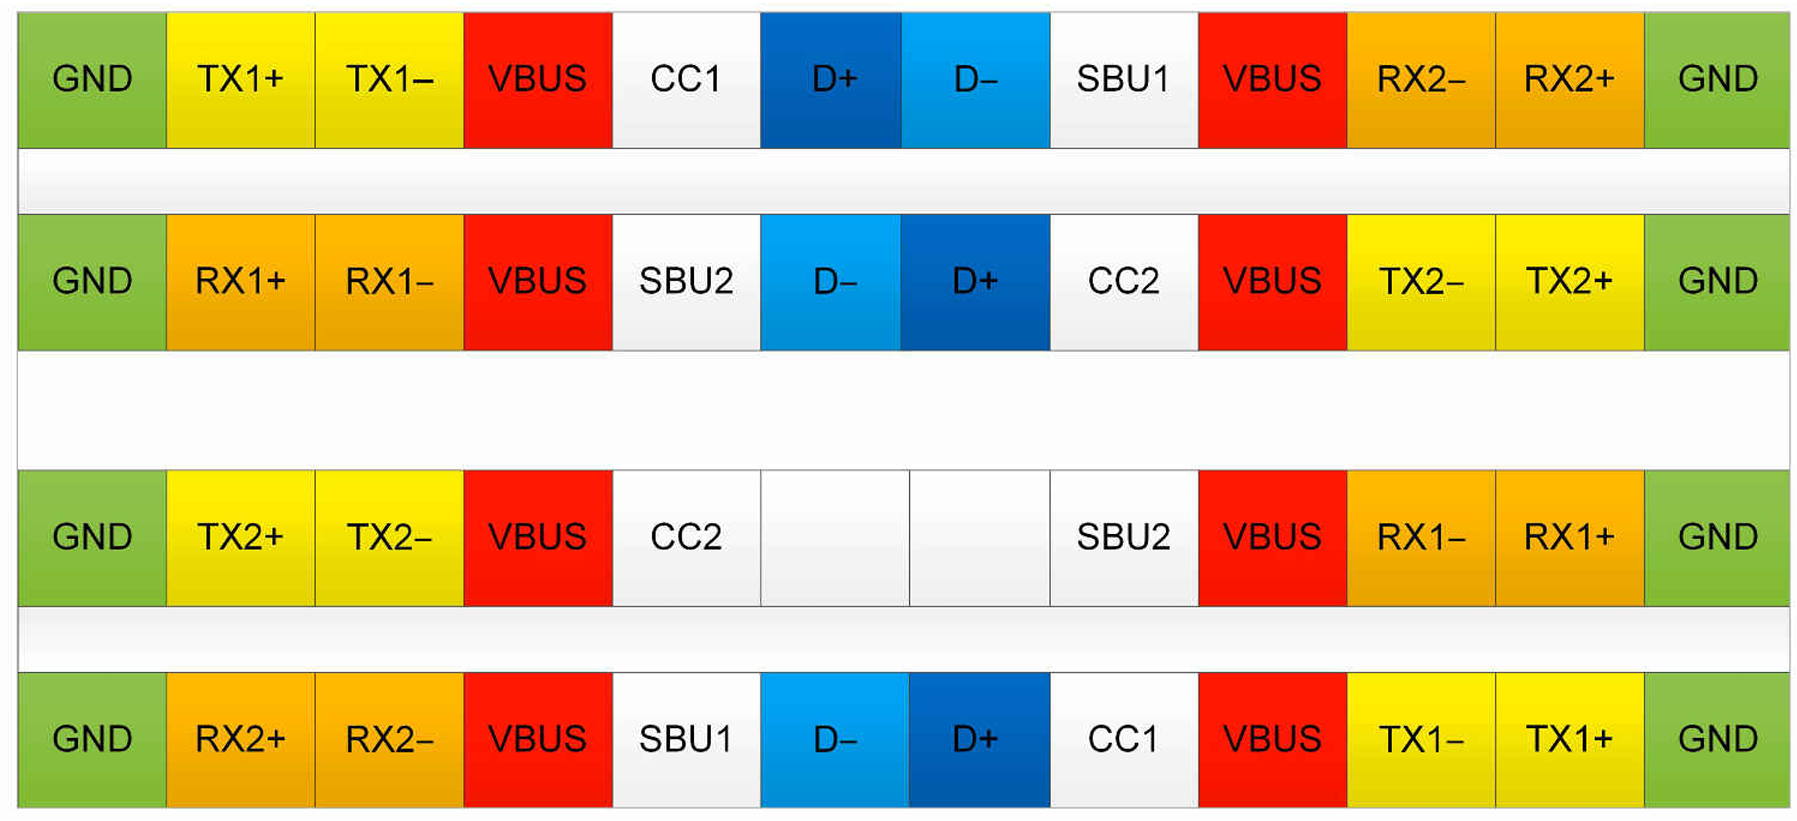
\includegraphics[width=0.7\linewidth]{Chapter2/typec_plugrecep.png}
    \caption{ Type-C pinout – receptacle (top), plug (bottom) \cite{enos2022primer}}
    \label{fig:typec_plug}
\end{figure}
The USB Type-C connector includes several new pins 
compared to USB Type-A and Type-B connectors. These 
pins enable USB Type-C features such as higher power, 
Alternate Mode and reversibility. Figure\ref{fig:typec_plug} illustrates the pinout.

From left to right \ref{fig:typec_plug} shows:
 \begin{enumerate}
     \item GND: the return path for the signal.
     \item TX/RX: SuperSpeed twisted pairs for USB 3.1 data (5 to 10 Gbps).
     \item VBUS: the main system bus (5 V to 20V).
     \item CC1/CC2: CC lines used for cable detection, orientation, and current advertisement. With USB PD, the CC lines can also communicate higher power levels and Alternate Mode. Note that one of the CC lines may become VCONN
     \item SBU1/SBU2: these are low-speed lines used only for Alternate Mode and accessory mode. For example, with DisplayPort, AUX+/AUX– transmit over the SBU lines. For audio adapter accessory mode, these lines are used for the microphone input and analog GND.
     \item D+/D–: a high-speed twisted pair for USB 2.0 data (up to 480 Mbps).
 \end{enumerate}
 It is observable that the GND and VBUS lines are still in the same position. The D+ / D– pair is in the same orientation; however, the plug contains only one D+ / D– twisted pair. The USB Type-C specification allows for the coupling of D+ / D- lines (D+ to D+ and D– to D–) on the receptacle side. Regardless of cable orientation, the PHY will always see the D+ / D- pair of the cable. 
 
 The CC1 and CC2 lines are flipped and can determine the orientation of the cable. The orientation determines which CC line is connected and which one is left open. The TX/RX pairs are also flipped. Resolving this was a bit more complicated. Unlike the D+/D– lines, you cannot simply short the common lines together, because that will create a stub. At USB 2.0 speeds, a stub is acceptable, but at USB 3.1 speeds, a stub degrades signal integrity too much.

 \subsection{Power Delivery}
 Applications with increasing complexity require USB PD. As mentioned in the introduction, systems with USB PD can support power levels of up to 20 V and 5 A (100 W). This is possible by first increasing the voltage on VBUS while holding the maximum current at 3 A. After reaching the maximum voltage of 20 V, you can increase the current up to 5 A, as seen in Figure\ref{fig:typec_power}.
 
\begin{figure}[htb]
\centering
	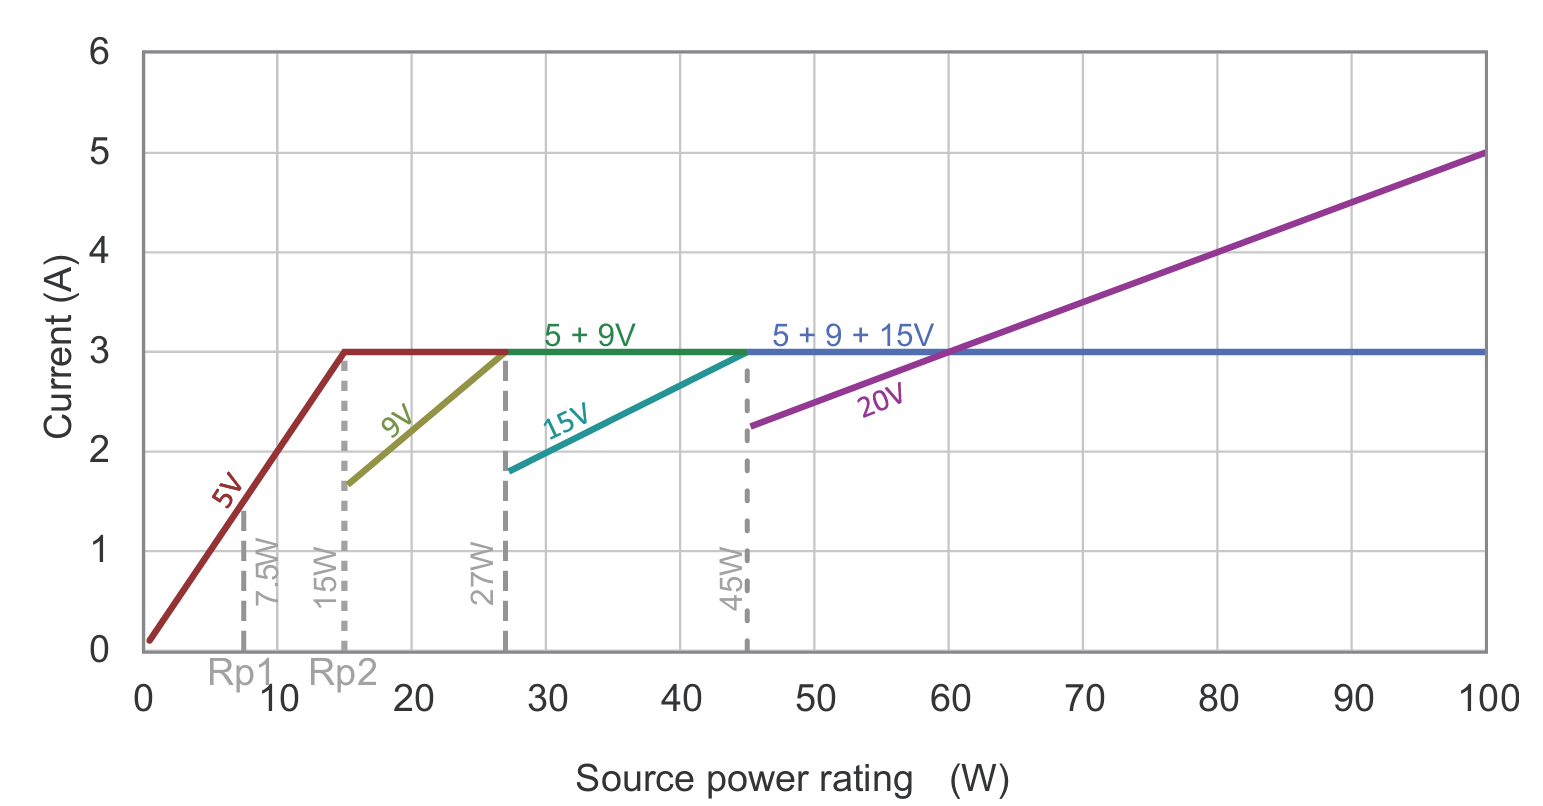
\includegraphics[scale=0.45]{Chapter2/PD_rating.png}	
	\caption{ USB PD profiles (power rails and maximum current) \cite{usb_power_delivery} }
	\label{fig:typec_power}
\end{figure}

Figure \ref{fig:typec_power} shows that, the discrete voltage levels required are 5 V, 9 V, 15 V and 20 V. The current can vary continuously, depending on the required power level (up to 3 A).  At any given power level, a source is required to support all previous voltages and power levels. For example, a 60-Watt source must be able to supply 5V at 3A, 9V at 3A, 15 V at 3A and 20 V at 3A. This is an update in version 3.0 of the USB PD specification, to ensure that higher power supplies could support lower powered devices. An example is a charger for both laptop, headphones, and mobile phone\cite{enos2022primer}.

\section{Standards and Protocols}

\gls{usbpd} specification defines how USB Devices can negotiate for more current and/or higher or lower Voltages over the USB cable (using the USB Type-C CC wire as the communications channel). It allows Devices with greater power requirements. In addition, it allows a Source and Sink to swap power roles such that a Device could supply power to the Host. For example, a display could supply power to a notebook to charge its battery \cite{usb_power_delivery}.

The USB Power Delivery Specification is guided by the following principles:
\begin{enumerate}
    \item Works seamlessly with legacy USB Devices.
    \item Optimized for low-cost implementations.
    \item Compatible with existing spec-compliant USB cables.
    \item Minimizes potential damage from non-compliant cables.
\end{enumerate}

\subsection{Source Operational Contracts}

A \gls{pd} Source will be in one of these three contracts:

\begin{enumerate}
    \item \textbf{Default Contract:} which it enters immediately following a connect where the Source provides 5V and advertises the amount of current it can deliver. A Source will remain in this Contract until the Sink is disconnected or the Source and Sink negotiate and enter an Explicit Contract.
    \item \textbf{Implicit Contract:} which is transitory and immediately follows a Power Role (PR) Swap.
    \item \textbf{Explicit Contract:} is the state of the Source after any PD power negotiation consisting of the Source sending a \textbf{Source Capabilities} Message, the Sink responding with a \textbf{Request} Message, the Source acknowledging the request with an \textbf{Accept} Message and finally the Source sends a \textbf{PS\_RDY} Message when the Source is ready to deliver the requested power. This is the normal operational state for PD.
\end{enumerate}

When Disconnected from the Sink, Source exits Explicit Contract. Source will restart in default state when reconnected to the Sink.

\subsection{USB Power Delivery Capable Devices}
\begin{figure}[hbt]
    \centering
    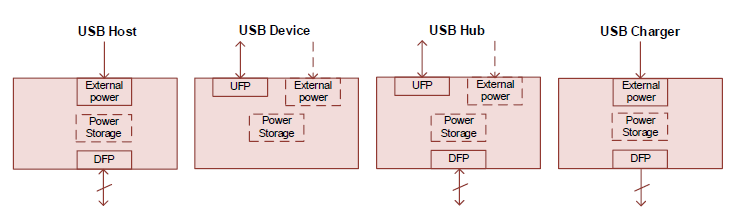
\includegraphics[width=0.8\linewidth]{Chapter2/pd_cap_dev.png}
    \caption{Logical Structure of USB Power Delivery Capable Devices}
    \label{fig:pd_cap_dev}
\end{figure}
As seen in Figure\ref{fig:pd_cap_dev}, each USB PD capable device is assumed to be made up of at least one Port. Providers are assumed to have a Source and Consumers a Sink. Each device contains one or more, of the following components:
\begin{enumerate}
    \item \gls{ufp}
    \item \gls{dfp}
    \item Source
    \item Sink
    \item VCONN Source
\end{enumerate}
UFPs, or Upstream Facing Ports, have several key characteristics. They are designed to sink power and communicate using SOP packets. Optionally, they can also communicate using SOP* packets. In addition to these functions, UFPs can optionally source power, making them a Dual-Role Power Device. They also have the capability to communicate via USB and support Alternate Modes.

DFPs, or Downstream Facing Ports, also have a range of features. They are primarily designed to source power and communicate using SOP packets. Like UFPs, they can optionally communicate using SOP* packets. DFPs can also optionally sink power, making them a Dual-Role Power Device as well. They have the option to communicate via USB and support Alternate Modes.

The source in this context can take several forms. It can be an externally powered source, such as an AC powered device. Alternatively, it can be a power storage device like a battery or power bank. It can also be derived from another port, such as a bus-powered hub.

A sink, on the other hand, can also be a power storage device like a battery or power bank. It can be used to power internal functions or to power devices attached to other devices, such as a bus-powered hub.

Lastly, a VCONN source has its own set of characteristics. It can be either port partner, either the DFP/UFP or Source/Sink. It powers the cable plug(s) and VPDs, or VCONN Powered Devices. Importantly, it is the only port allowed to talk to the cable plug(s) at any given time. This ensures a clear and uninterrupted communication pathway.
\vspace{3cm}
%\section{LDMOS and GaN HEMTs : A Comparison of Power MOSFETs}
 